% Chapter 3

\chapter{CONCEPTUAL FRAMEWORK} % Main chapter title

\label{Chapter3} % Change X to a consecutive number; for referencing this chapter elsewhere, use \ref{ChapterX}

\lhead{Chapter 3. \emph{Conceptual Framework}} % Change X to a consecutive number; this is for the header on each page - perhaps a shortened title

%----------------------------------------------------------------------------------------
%	SECTION 1
%----------------------------------------------------------------------------------------



%\begin{figure}[htbp]
%	\centering
%	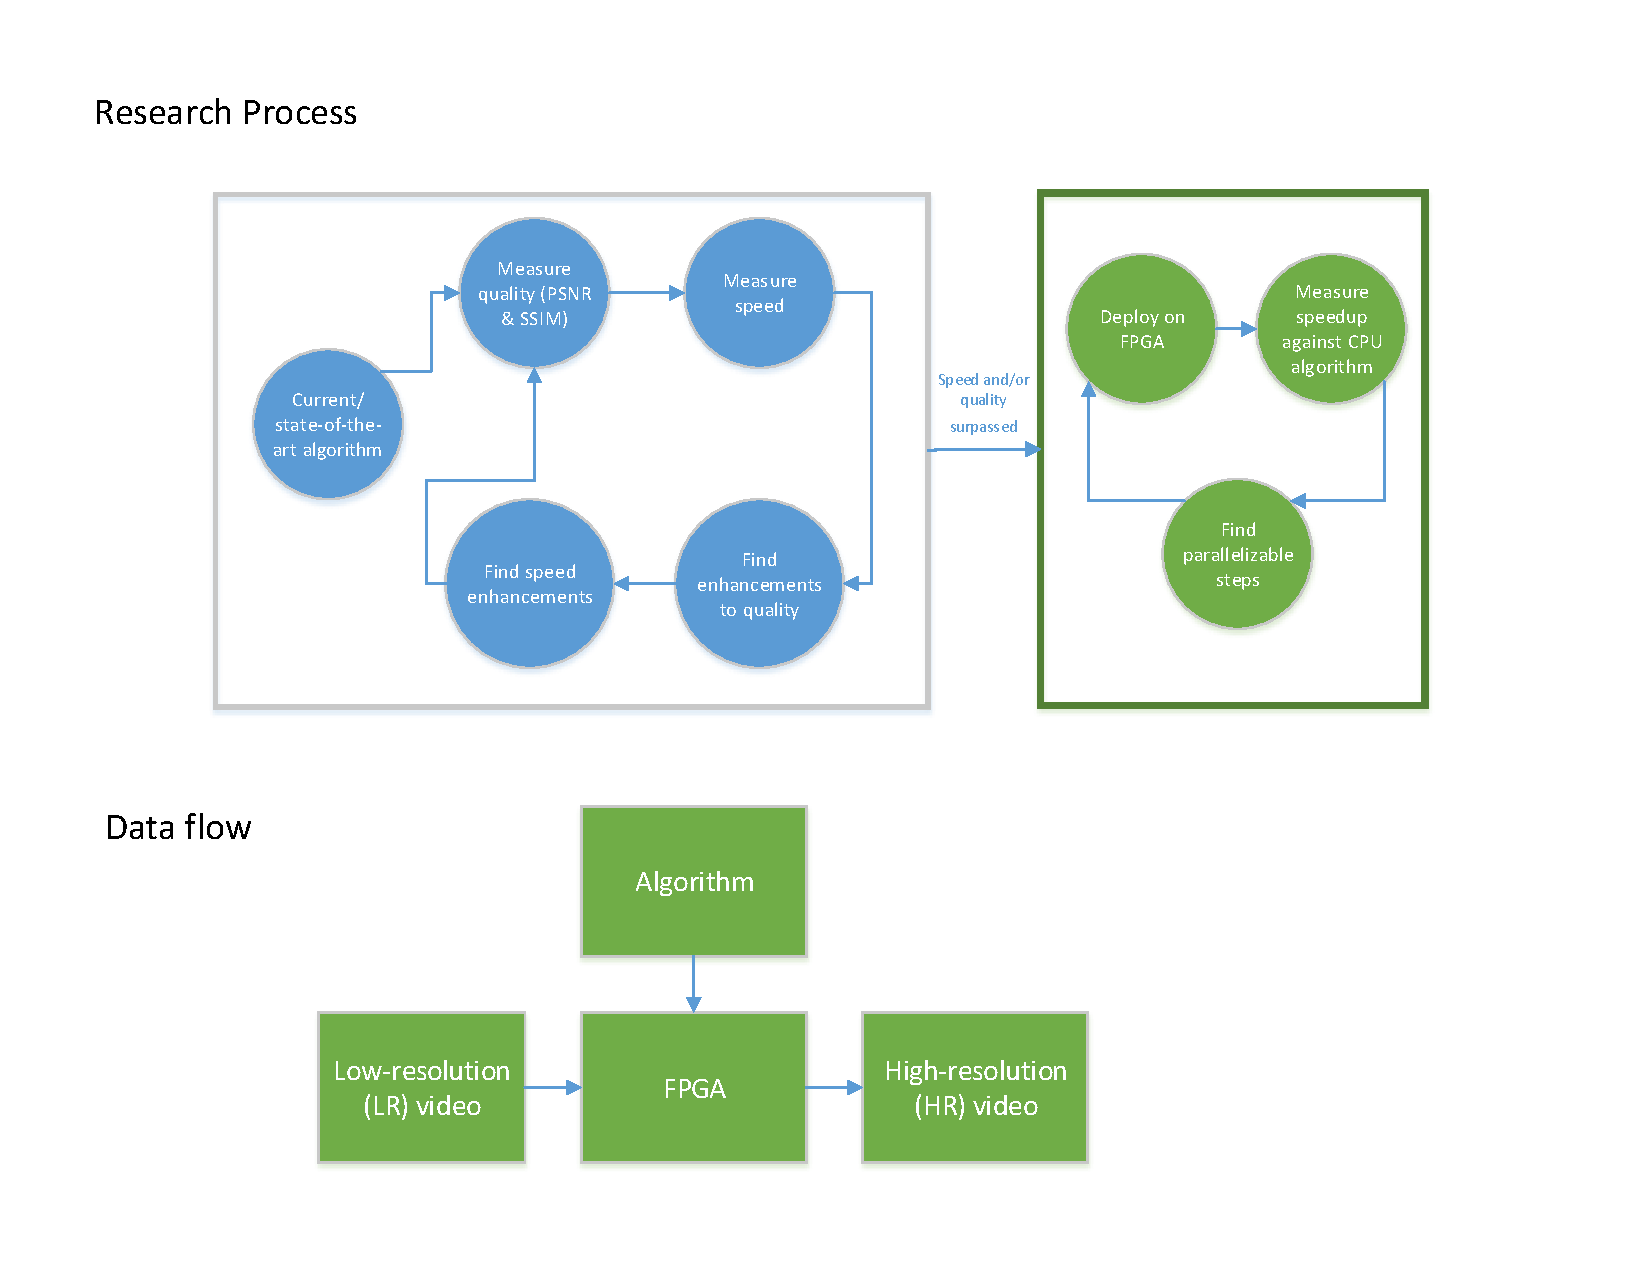
\includegraphics{Figures/framework.pdf}
%	\rule{35em}{0.2pt}
%	\caption[Conceptual Framework]{Conceptual Framework of the Study.}
%	\label{fig:Framework}
%\end{figure}



%-----------------------------------
%	SUBSECTION 1
%-----------------------------------
\section{Algorithm Framework}
% Place figure here

% Explain the framework

%-----------------------------------
%	SUBSECTION 2
%-----------------------------------

\section{Hardware Framework}
\begin{figure}
	\centering
	\includegraphics[scale=0.5]{Figures/HARDWARE_FRAMEWORK.png}
	\caption[]{Framework for Hardware Implementation.}
	\label{fig:hardframe}
\end{figure}

% Explain the framework
Figure \ref{fig:hardframe} illustrates the flow of data across the hardware devices to be used in the study.
A video source such as a camera or prerecorded file will be sent for super-resolution on the SoC, which will then display the result on the monitor in real-time.
Initially a conventional computer will serve as the development and evaluation  environment for the SR algorithm.
A revised version of the algorithm can then be sent to the SoC for further testing and fine-tuning.



%----------------------------------------------------------------------------------------
%	SECTION 2
%----------------------------------------------------------------------------------------
